\level{1}{Bugs report and new features request}
If you want to report bugs or ask for new features, you can do it from \insglo{Norris}' repository on Github. Just follow these steps:
\begin{enumerate}
	\item open \insglo{Norris}' repository, you can find it at \insuri{};
	\item go to “Issues” link, you can find it on the right side of the page;
	\begin{figure}[H]
		\centering
		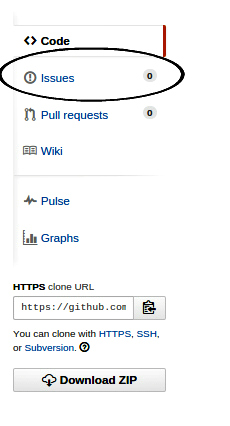
\includegraphics[scale=0.6]{Pics/Issues.jpg}
		\caption{Click on “Issues” link to view all issues open}
	\end{figure}
	\item before submitting any request, please, see if this bug or enhancement has already been reported;
	\item if not, add a new issue, by clicking on “New issue” button;
	\begin{figure}[H]
		\centering
		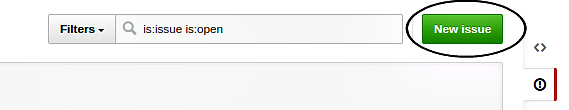
\includegraphics[scale=0.6]{Pics/NewIssue.jpg}
		\caption{Click on “New issue” button to open a new issue}
	\end{figure}
	\item set the title of the issue, make sure it's concise and descripted;
	\item describe the problem (if you're reporting a bug), providing as much information as possible in order for us to reproduce it and solve it;
	\begin{figure}[H]
		\centering
		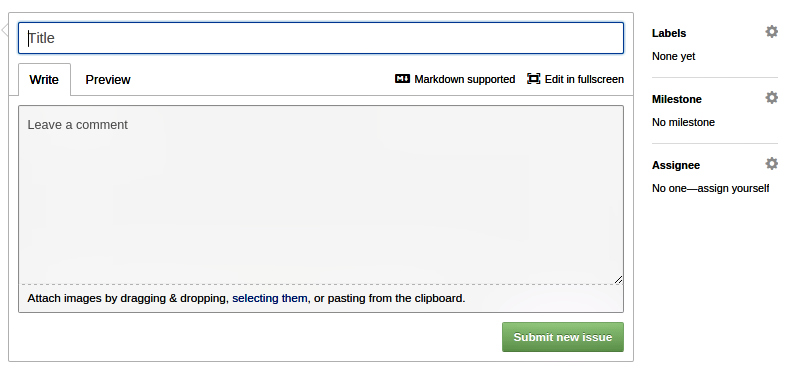
\includegraphics[scale=0.6]{Pics/TextIssue.jpg}
		\caption{Write a new issue}
	\end{figure}
	\item if you want to request new features, try to make a complete description of your request;
	\item set the right label (“bug”, “enhancement”), to facilitate the tracking of the new issue, and submite it.
	\begin{figure}[H]
		\centering
		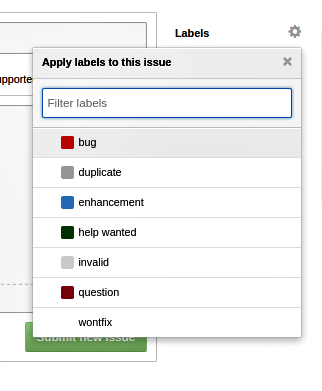
\includegraphics[scale=0.6]{Pics/Labels.jpg}
		\caption{Set the issue's labels}
	\end{figure}
\end{enumerate}

An activity diagram, riassuming this procedure, follows.
\begin{figure}[H]
	\centering
	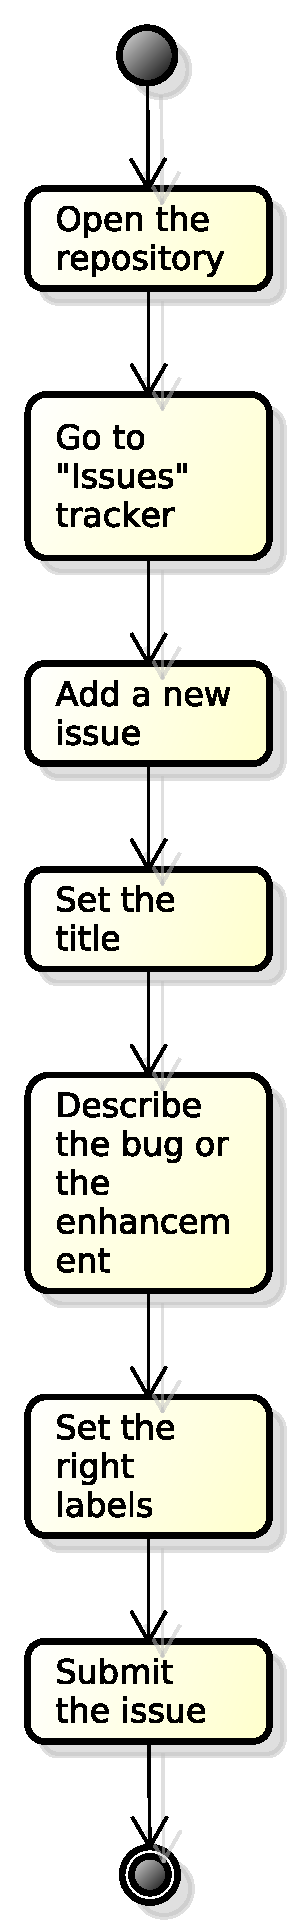
\includegraphics[scale=0.4]{Pics/ReportIssue.pdf}
	\caption{How to report a bug or request new features}
\end{figure}
